%% ------------------------------------------------------------------------
%% DER-SafeAgent — Supplementary Material (IJCIP final revision)
%% Compile independently:  tectonic supplementary.tex
%% ------------------------------------------------------------------------
\documentclass[11pt,a4paper]{article}
\usepackage[utf8]{inputenc}
\usepackage[T1]{fontenc}
\usepackage{lmodern}
\usepackage{graphicx}
\usepackage{amsmath,amssymb}
\usepackage{booktabs}
\usepackage{verbatim}
\usepackage{url}
\usepackage{xcolor}
\usepackage{tabularx}
\usepackage{xltabular}
\usepackage[margin=2.4cm]{geometry}
\usepackage[hidelinks]{hyperref}

\providecommand{\ours}{\textsc{DER-SafeAgent}}
% macros used by the reused revision tables
% Auto-generated by code/evaluation/build_revision_artifacts.py.
% Do not edit by hand -- regenerate from the raw result files.
\newcommand{\nStubConfigs}{25}
\newcommand{\nStubAttackConfigs}{24}
\newcommand{\nDssConfigs}{20}
\newcommand{\nDssRows}{60}
\newcommand{\HypLatKOne}{$4.7$\,s}
\newcommand{\HypLatKThree}{$5.6$\,s}
\newcommand{\CautionLat}{$\sim$$2$\,s}
\newcommand{\ColdStart}{$\sim$$10$\,s}
\newcommand{\REVresultsAbstract}{The deterministic safety-policy configuration and the real Qwen QLoRA-in-the-loop configuration reach mean ENS of $3.19$ and $3.19$\,kWh respectively over the evaluated library; across 29 model-consulted decision steps the safety layer changed the model's proposed action at 10 of them, and the irreversible \texttt{isolate\_inverter} primitive was proposed 2 times but executed 0 times.}


\title{Supplementary Material for\\
\emph{DER-SafeAgent: A Runtime-Assurance Architecture for Safe
LLM-Assisted Cyber-Physical Incident Response in Distributed Energy
Resources}}
\date{}

\begin{document}
\maketitle

\noindent This supplement contains material referenced from the main
manuscript. The main manuscript is self-contained; nothing here is
required to follow its argument. Naming note: the system was renamed from
\textsc{DER-SecAgent} to \textsc{DER-SafeAgent} at the final revision;
the code repository, module paths, and historical result directories
retain the legacy name for reproducibility, and all repository paths
cited below are unchanged.

\tableofcontents

\renewcommand{\thesection}{S\arabic{section}}
% The reused appendix sources begin with \appendix; make it harmless here
% so S-numbering is preserved.
\renewcommand{\appendix}{}

%% S1–S2 reuse the previous appendix sources verbatim.
\appendix
\section{Prompts and Agent Schemas}
% Reviewer hooks: R2.C5, R3.C7
%
% This appendix reproduces verbatim every prompt used in the paper, so the
% study is fully reproducible. Each listing prints its file path, byte
% length, and SHA-256 hash; the same hashes are recorded in run manifests
% per docs/reproducibility.md.

\paragraph{Reproducibility note}
The hashes printed beneath each listing are the values produced by
``sha256sum'' on the file contents at submission time. Runs will refuse
to start if the runtime hash does not match the manifest hash, so any
post-submission editing of these prompts can be detected automatically.

\subsection*{A.1 Single-LLM baseline prompt}
\label{ssec:prompt-single-llm}
File: \texttt{code/baselines/single\_llm/prompt.txt} \\
SHA-256: {\small\texttt{49fff5dcd3b3b12ec71bdb4b85de01f23de777802895ad0acbe1ea4b963e79ac}}
\begin{small}
\verbatiminput{listings/single_llm_prompt.txt}
\end{small}

\subsection*{A.2 Hypothesis Agent prompt (DER-SecAgent)}
\label{ssec:prompt-hypothesis}
File: \texttt{code/Multi\_AI\_Agent/prompts/hypothesis.txt} \\
SHA-256: {\small\texttt{b3012fae512e7deafd3e0fecb007c0ac76b22620c27c186191c8f47ffdf0501f}}
\begin{small}
\verbatiminput{listings/hypothesis.txt}
\end{small}

\subsection*{A.3 Energy Impact Agent prompt}
\label{ssec:prompt-energy}
File: \texttt{code/Multi\_AI\_Agent/prompts/energy\_estimator.txt} \\
SHA-256: {\small\texttt{6bb31180b347b65812a4d69abe5b84ddb8e122695ee3cc51ac70be8ff28529d0}}
\begin{small}
\verbatiminput{listings/energy_estimator.txt}
\end{small}

\subsection*{A.4 Caution Agent prompt}
\label{ssec:prompt-caution}
File: \texttt{code/Multi\_AI\_Agent/prompts/caution.txt} \\
SHA-256: {\small\texttt{798d1148b24985b37527c8dd5d28290db7a117482cf4f62c55d04fc88edbd17b}}
\begin{small}
\verbatiminput{listings/caution.txt}
\end{small}

\subsection*{A.5 Coordinator (Critic) Agent prompt}
\label{ssec:prompt-coordinator}
File: \texttt{code/Multi\_AI\_Agent/prompts/coordinator.txt} \\
SHA-256: {\small\texttt{a8cf8133cb0c6300a318f372a573ce10be91bb1617512cad388398fac7907114}}
\begin{small}
\verbatiminput{listings/coordinator.txt}
\end{small}

\subsection*{A.6 Report Agent prompt and JSON schema}
\label{ssec:prompt-report}
File: \texttt{code/Multi\_AI\_Agent/prompts/report.txt} \\
SHA-256: {\small\texttt{d68d2778d4d3f27b33659d84459a27515b9fc6470bb3b7a8be91a47e96c0270b}}
\begin{small}
\verbatiminput{listings/report.txt}
\end{small}

\subsection*{A.7 Strategy hint templates}
\label{ssec:prompt-strategy}
\paragraph{Chain-of-Thought hint}
File: \texttt{code/Multi\_AI\_Agent/prompts/cot.txt} \\
SHA-256: {\small\texttt{2536b39f42c9524ec019f372c34d5b5b0dd9ff6ae3bc24a2b96635a6b62043ce}}
\begin{small}
\verbatiminput{listings/cot.txt}
\end{small}

\paragraph{Tree-of-Thought hint}
File: \texttt{code/Multi\_AI\_Agent/prompts/tot.txt} \\
SHA-256: {\small\texttt{3371065aeae55cf62554b4c115648bfd730b38d755e0db6b8035832af2956e86}}
\begin{small}
\verbatiminput{listings/tot.txt}
\end{small}

\paragraph{Few-shot exemplars}
The four held-in exemplars used by the Few-shot variant are
\texttt{syn-00000}, \texttt{syn-00001}, \texttt{syn-00002}, and
\texttt{syn-00009} from the train split of the v0.1 corpus
(SHA-256 of \texttt{train.jsonl}:
\texttt{9de44c2780c9a8ab2baffa8517faab4ac9350797b9aa36734730deb3257b4845};
see Data Card). Each is a one-turn (user, assistant) pair conforming
to the Hypothesis Agent schema.

\subsection*{A.8 Judge prompt and scoring rubric}
\label{ssec:prompt-judge}
File: \texttt{code/Multi\_AI\_Agent/prompts/judge.txt} \\
SHA-256: {\small\texttt{c19f0fc249000222aa18525edaf4d997f3682c7079940154cae7426eb209e270}}
\begin{small}
\verbatiminput{listings/judge.txt}
\end{small}

\section{LangGraph State Schema and Inter-Agent Contract}
\label{sec:appendix-state}
% Reviewer hooks: R3.C7
%
% Reproduces the TypedDict schema used to pass state between the five
% agents (plus the post-hoc Report Agent). The source of truth is
% code/Multi_AI_Agent/states.py; this appendix is a verbatim listing.

\paragraph{Source}
The schema is defined as a Python \texttt{TypedDict} in
\texttt{code/Multi\_AI\_Agent/states.py}; the verbatim listing follows.
Inter-agent communication is by mutation of a single
\texttt{AgentState} dictionary, which both keeps the LangGraph
state-machine declarative and lets the harness persist a complete decision
record per invocation.

\begin{small}
\verbatiminput{listings/states.py}
\end{small}

\paragraph{Field ownership}
The 2026 v2 fields added on top of the 2025 schema are owned by exactly
one agent each, so a transcript of the state at any node boundary is
sufficient to attribute every value to a producer:

\begin{tabular}{lll}
\toprule
Field & Producer & Consumers \\
\midrule
\texttt{feature\_view}        & Telemetry Analyst & Hypothesis, Energy, Coordinator \\
\texttt{hypothesis}           & Hypothesis Agent  & Caution, Coordinator \\
\texttt{attack\_class}        & Hypothesis Agent  & Caution, Coordinator, harness \\
\texttt{confidence}           & Hypothesis Agent  & Caution, Coordinator, harness \\
\texttt{proposed\_action}     & Hypothesis Agent  & Caution, Coordinator (informational) \\
\texttt{expected\_impact\_tier}& Hypothesis Agent & Caution \\
\texttt{impact\_estimates}    & Energy Impact Ag. & Coordinator \\
\texttt{caution}              & Caution Agent     & Coordinator \\
\texttt{caution\_reason}      & Caution Agent     & Coordinator, audit \\
\texttt{final\_action}        & Coordinator       & harness, audit \\
\texttt{final\_action\_target}& Coordinator       & harness, audit \\
\texttt{final\_impact\_tier}  & Coordinator       & audit \\
\texttt{coordinator\_decision}& Coordinator       & harness (HITL routing) \\
\texttt{coordinator\_reason}  & Coordinator       & audit \\
\texttt{chosen\_for\_hitl}    & Coordinator       & HITL operator \\
\texttt{decision\_id}         & Hypothesis Agent  & Report, audit \\
\texttt{report}               & Report Agent      & audit (hash-chain) \\
\bottomrule
\end{tabular}

\paragraph{Topology}
The LangGraph topology is built in
\texttt{code/Multi\_AI\_Agent/build\_graph.py}; the v2 pipeline runs as
\textsc{Telemetry Analyst} $\to$ \textsc{Hypothesis} $\to$
\textsc{Energy Impact} $\to$ \textsc{Caution} $\to$
\textsc{Coordinator} $\to$ END, with the Report Agent invoked
post-hoc per resolved incident.


\section{Operational definition of trustworthiness}
\label{sec:supp-trustworthy}
Table~\ref{tab:trustworthy} gives the full operational definition of
``trustworthy'' as used in the main text: for each property, the implementation
mechanism, how it is evaluated and the supporting evidence, and the remaining
limitation.
% Auto-generated by code/evaluation/build_revision_artifacts.py
% (hand-tightened for IJCIP: the original seven columns did not fit the text
%  width, so evaluation method, metric, and evidence are merged into one
%  "Evaluation & evidence" column; the table is a page-breaking xltabular set
%  in scriptsize so all seven rows appear without clipping.)
{\scriptsize
% Long \texttt{...} identifiers are made breakable at underscores so no cell
% overflows its column edge.
\renewcommand{\_}{\char`\_\allowbreak}
\renewcommand{\arraystretch}{1.15}
\begin{xltabular}{\textwidth}{@{}>{\raggedright\arraybackslash}p{0.92in}
 >{\raggedright\arraybackslash}X >{\raggedright\arraybackslash}X
 >{\raggedright\arraybackslash}X >{\raggedright\arraybackslash}X@{}}
\caption{Operational definition of \emph{trustworthy} as used in this paper.
Trustworthiness here denotes the implemented and empirically evaluated
properties below, not a formal or universal safety guarantee. Each row names
the mechanism, how it is evaluated and the evidence, and the limitation that
remains.}\label{tab:trustworthy}\\
\toprule
Characteristic & Operational definition & Implementation mechanism & Evaluation \& evidence & Known limitation \\
\midrule
\endfirsthead
\multicolumn{5}{@{}l}{\emph{Table~\ref{tab:trustworthy} (continued)}}\\[2pt]
\toprule
Characteristic & Operational definition & Implementation mechanism & Evaluation \& evidence & Known limitation \\
\midrule
\endhead
\midrule
\multicolumn{5}{r@{}}{\emph{continued on next page}}\\
\endfoot
\bottomrule
\endlastfoot
\textbf{Boundedness} & Executable action $\in$ fixed five-primitive registry; no free-form commands. & Registry + enum/schema validation at the pipeline boundary (\texttt{mitigations.py}). & Registry / coordinator unit tests; forbidden-action and in-registry rates; 7 tests + adversarial suite. & Registry fixed at design time; a novel required action is inexpressible. \\
\addlinespace[2pt]
\textbf{Robustness} & Injected instructions / poisoned memory do not change the executed action (tested suite). & Deterministic FeatureView; Evidence Gate; schema; class-aware projection; irreversible $\Rightarrow$ escalate. & 14-family adversarial suite; policy-violation, safe-fallback, proposed-vs-final divergence rates. & Empirical, tested suite only; not a guarantee vs.\ adaptive white-box attackers. \\
\addlinespace[2pt]
\textbf{Human oversight} & Low-confidence, high-impact actions withheld and routed to an operator. & Caution Agent + Coordinator HITL gate + ChatOps SLO / expiry fallback. & HITL sensitivity study + gate unit tests; escalation, SLO-expiry, unsafe-command rates. & Operators are deterministic stand-ins, not human subjects. \\
\addlinespace[2pt]
\textbf{Traceability} & Post-hoc edit, deletion, or reordering is detectable relative to a trusted stored chain head. & Deterministic SHA-256 hash chain (\texttt{audit\_chain.py}), outside model control. & Chain verification vs a stored head: tamper / delete / reorder tests; pass/fail and first-broken index. & Detects edits vs a stored head only; no origin authentication, timestamping, or protection against full recomputation by an attacker controlling the whole log. \\
\addlinespace[2pt]
\textbf{Reliability} & Same input window $\rightarrow$ same features and same deterministic path. & Deterministic FeatureView; greedy decoding; optional $K{=}3$ self-consistency. & Determinism + repeated-configuration tests; byte-identical reproduction, vote share, abstention rate. & LLM stage only as reliable as the model; JSON validity $<1.0$ observed. \\
\addlinespace[2pt]
\textbf{Cyber-physical safety awareness} & Action accounts for energy consequence and attack-class physics. & Holdout-validated EH estimator ranks safe fallback; class-aware projection. & StubFeeder and real OpenDSS sweeps; ENS, curtailed energy, voltage min/max and violation fraction, ramp violations. & Simulation only; StubFeeder voltage is a proxy, so voltage claims rest on OpenDSS. \\
\addlinespace[2pt]
\textbf{Fail-safe behaviour} & Model unavailable / slow / unparseable $\Rightarrow$ still a bounded conservative action. & \texttt{no\_op} / \texttt{freeze\_setpoint} fallback; SLO-expiry fallback; strict-mode abort. & Strict-mode + deadline-aware tests; fallback rate and incidents resolved before each SLO. & Bounded but not always optimal; a wrong-but-safe action still curtails energy. \\
\end{xltabular}
\par}


\section{Complete scenario and configuration manifests}
The frozen 25-configuration cyber-physical library is defined by
\texttt{code/configs/ijcip\_revision\_r1r2\_20260805/scenario\_manifest.csv}
(SHA-256 per configuration). The final-revision additions
(tag \texttt{ijcip\_final\_safeagent\_20260810}) are:
the 12-configuration estimator holdout
(\texttt{impact\_estimator\_holdout.csv}),
the 32-configuration Evidence-Gate test set
(\texttt{evidence\_gate\_test.csv}),
and the 12-configuration pre-registered OpenDSS subset
(\texttt{opendss\_llm\_subset.csv});
each manifest carries per-file SHA-256 hashes and a freeze note recording
that it was written before the corresponding evaluation.
% Auto-generated by code/evaluation/build_revision_artifacts.py
\begin{table*}[t]
\centering
\caption{Expanded StubFeeder scenario library (25 unique configurations,
of which 1 is a benign calibration control excluded from the primary
significance analysis). Configurations vary causal factors, not random seeds:
the harness is deterministic given a configuration, so each configuration is run
once and the \emph{configuration} is the unit of statistical inference. The
manifest is frozen (SHA-256 recorded in
\texttt{code/configs/ijcip\_revision\_r1r2\_20260805/scenario\_matrix.yaml}).}
\label{tab:scenario-matrix}
\scriptsize
\setlength{\tabcolsep}{3pt}
\begin{tabular}{@{}p{0.34\textwidth}llllll@{}}
\toprule
Scenario ID & Attack & Mag. & Duration & Load & DER pen. & Asset \\
\midrule
\texttt{\scriptsize 13:fdi\_med\_medium\_nom\_medpen\_inv} & fdi & med & medium & nominal & med & INV\_634 \\
\texttt{\scriptsize 13:spoof\_med\_medium\_nom\_medpen\_inv} & command\_spoof & med & medium & nominal & med & INV\_634 \\
\texttt{\scriptsize 13:replay\_med\_medium\_nom\_medpen\_inv} & replay & med & medium & nominal & med & INV\_634 \\
\texttt{\scriptsize 13:dos\_med\_medium\_nom\_medpen\_inv} & dos & med & medium & nominal & med & INV\_634 \\
\texttt{\scriptsize 13:fdi\_low\_medium\_nom\_medpen\_inv} & fdi & low & medium & nominal & med & INV\_634 \\
\texttt{\scriptsize 13:fdi\_high\_medium\_nom\_medpen\_inv} & fdi & high & medium & nominal & med & INV\_634 \\
\texttt{\scriptsize 13:spoof\_low\_medium\_nom\_medpen\_inv} & command\_spoof & low & medium & nominal & med & INV\_634 \\
\texttt{\scriptsize 13:spoof\_high\_medium\_nom\_medpen\_inv} & command\_spoof & high & medium & nominal & med & INV\_634 \\
\texttt{\scriptsize 13:dos\_med\_short\_nom\_medpen\_inv} & dos & med & short & nominal & med & INV\_634 \\
\texttt{\scriptsize 13:dos\_med\_persistent\_nom\_medpen\_inv} & dos & med & persistent & nominal & med & INV\_634 \\
\texttt{\scriptsize 13:spoof\_med\_short\_nom\_medpen\_inv} & command\_spoof & med & short & nominal & med & INV\_634 \\
\texttt{\scriptsize 13:spoof\_med\_persistent\_nom\_medpen\_inv} & command\_spoof & med & persistent & nominal & med & INV\_634 \\
\texttt{\scriptsize 13:spoof\_med\_medium\_light\_medpen\_inv} & command\_spoof & med & medium & light & med & INV\_634 \\
\texttt{\scriptsize 13:spoof\_med\_medium\_peak\_medpen\_inv} & command\_spoof & med & medium & peak & med & INV\_634 \\
\texttt{\scriptsize 13:fdi\_med\_medium\_peak\_medpen\_inv} & fdi & med & medium & peak & med & INV\_634 \\
\texttt{\scriptsize 13:dos\_med\_medium\_light\_medpen\_inv} & dos & med & medium & light & med & INV\_634 \\
\texttt{\scriptsize 13:spoof\_med\_medium\_nom\_lowpen\_inv} & command\_spoof & med & medium & nominal & low & INV\_634 \\
\texttt{\scriptsize 13:spoof\_med\_medium\_nom\_highpen\_inv} & command\_spoof & med & medium & nominal & high & INV\_634 \\
\texttt{\scriptsize 13:fdi\_med\_medium\_nom\_lowpen\_inv} & fdi & med & medium & nominal & low & INV\_634 \\
\texttt{\scriptsize 13:spoof\_med\_medium\_nom\_medpen\_bess} & command\_spoof & med & medium & nominal & med & BESS\_675 \\
\texttt{\scriptsize 34:spoof\_high\_medium\_nom\_medpen\_inv840} & command\_spoof & high & medium & nominal & med & INV\_840 \\
\texttt{\scriptsize 34:spoof\_high\_medium\_nom\_medpen\_fleet} & command\_spoof & high & medium & nominal & med & fleet INV\_840+INV\_824 \\
\texttt{\scriptsize 34:dos\_med\_persistent\_nom\_medpen\_bess848} & dos & med & persistent & nominal & med & BESS\_848 \\
\texttt{\scriptsize 13:benign\_none\_none\_nom\_medpen\_none} & none & none & none & nominal & med & none \\
\texttt{\scriptsize 13:replay\_high\_medium\_nom\_medpen\_inv} & replay & high & medium & nominal & med & INV\_634 \\
\bottomrule
\end{tabular}
\end{table*}


\section{Full QLoRA evaluation}
Expanded QLoRA corpus results (146 leakage-controlled prompts per
backbone), calibration and confusion detail, and the $K{=}1$ vs $K{=}3$
comparison.
% Auto-generated by code/finetuning_dataset/revision_eval/analyse_eval.py
\begin{table*}[t]
\centering
\caption{Expanded QLoRA evaluation on the leakage-controlled corpus. Prompts
are stratified across the six in-taxonomy classes and eight families
(scenario-derived, paraphrased alerts, conflicting telemetry, malformed alerts,
prompt injection, memory poisoning, out-of-distribution labels, and
benign-but-suspicious). A two-part duplicate filter was applied before any
model was run: a leakage filter comparing digit-masked text against every
training, validation and test prompt, and a diversity filter on unmasked
5-grams against accepted candidates. Expected labels and expected safe actions
come from scenario ground truth or the deployed class-to-action registry and
were fixed before inference. ``Proposed'' is the model's own action; ``final''
is the action after the class-aware avoidance set and Caution gate --- the gap
between them is safety containment, not model skill. The three right-hand
columns separate failure modes that a single ``forbidden-action rate''
conflates: \emph{out-of-registry} (an executed action outside the five
primitives --- the invariant the action surface must make impossible),
\emph{class-inappropriate} (a registry action on the avoidance list for the
predicted class, which the class-aware avoidance set exists to prevent), and
\emph{false-positive action} (the incident is benign but the model asserted an
attack, so any action is unnecessary curtailment --- a limit of the safety
layer, which bounds \emph{which} action is taken but cannot decide that no
incident exists). ``Irrev.'' counts how often the irreversible
\texttt{isolate\_inverter} primitive was proposed versus executed. Brackets
are bootstrap 95\% CIs.}
\label{tab:lora-eval-expanded}
\scriptsize
\setlength{\tabcolsep}{3pt}
\begin{tabular}{@{}llrccccccccccc@{}}
\toprule
Backbone & $K$ & $n$ & Class acc.\ [95\% CI] & Macro-F1 & Prop.\ act. & Final act. & JSON & Schema & Out-of-reg. & Class-inapp. & False-pos.\ act. & Irrev.\ prop./exec. & Lat.\ (s) \\
\midrule
llama3\_1\_8b\_lora & $K{=}1$ & 146 & 0.418 [0.34,0.50] & 0.407 & 0.384 & 0.610 & 1.000 & 0.753 & 0.000 & 0.000 & 0.196 & 6/0 & 5.6 \\
llama3\_1\_8b\_lora & $K{=}3$ & 48 & 0.521 [0.38,0.67] & 0.553 & 0.479 & 0.667 & 1.000 & 0.833 & 0.000 & 0.000 & 0.000 & 0/0 & 17.4 \\
qwen2\_5\_7b\_lora & $K{=}1$ & 146 & 0.404 [0.33,0.49] & 0.359 & 0.377 & 0.658 & 1.000 & 0.692 & 0.000 & 0.000 & 0.137 & 14/0 & 5.4 \\
qwen2\_5\_7b\_lora & $K{=}3$ & 48 & 0.542 [0.40,0.67] & 0.425 & 0.646 & 0.708 & 1.000 & 0.917 & 0.000 & 0.000 & 0.222 & 0/0 & 16.8 \\
\bottomrule
\end{tabular}
\end{table*}

% Auto-generated by code/finetuning_dataset/revision_eval/compare_k.py
\begin{table}[t]
\centering
\caption{$K{=}1$ versus $K{=}3$ self-consistency, compared only on the
prompts both settings saw (the $K{=}3$ runs use the pre-registered subset, so
comparing against full-corpus $K{=}1$ numbers would confound the $K$ setting
with prompt difficulty). ``Agree'' counts prompts on which the two settings
predict the same attack class --- the quantity that decides whether
self-consistency is doing any work. ``Irrev.'' is the irreversible
\texttt{isolate\_inverter} primitive, proposed / executed.}
\label{tab:k1-vs-k3}
\scriptsize
\setlength{\tabcolsep}{4pt}
\begin{tabular}{llrccccccc}
\toprule
Backbone & $K$ & $n$ & Class acc. & Prop.\ act. & Final act. & Schema & Lat.\ (s) & Irrev. & Agree \\
\midrule
qwen2\_5\_7b\_lora & $K{=}1$ & 48 & 0.500 & 0.583 & 0.667 & 0.896 & 5.6 & 0/0 &  \\
 & $K{=}3$ & 48 & 0.542 & 0.646 & 0.708 & 0.917 & 16.8 & 0/0 & 45/48 \\
llama3\_1\_8b\_lora & $K{=}1$ & 48 & 0.500 & 0.521 & 0.667 & 0.812 & 5.6 & 0/0 &  \\
 & $K{=}3$ & 48 & 0.521 & 0.479 & 0.667 & 0.833 & 17.4 & 0/0 & 43/48 \\
\bottomrule
\end{tabular}
\end{table}

\begin{figure}[h]\centering
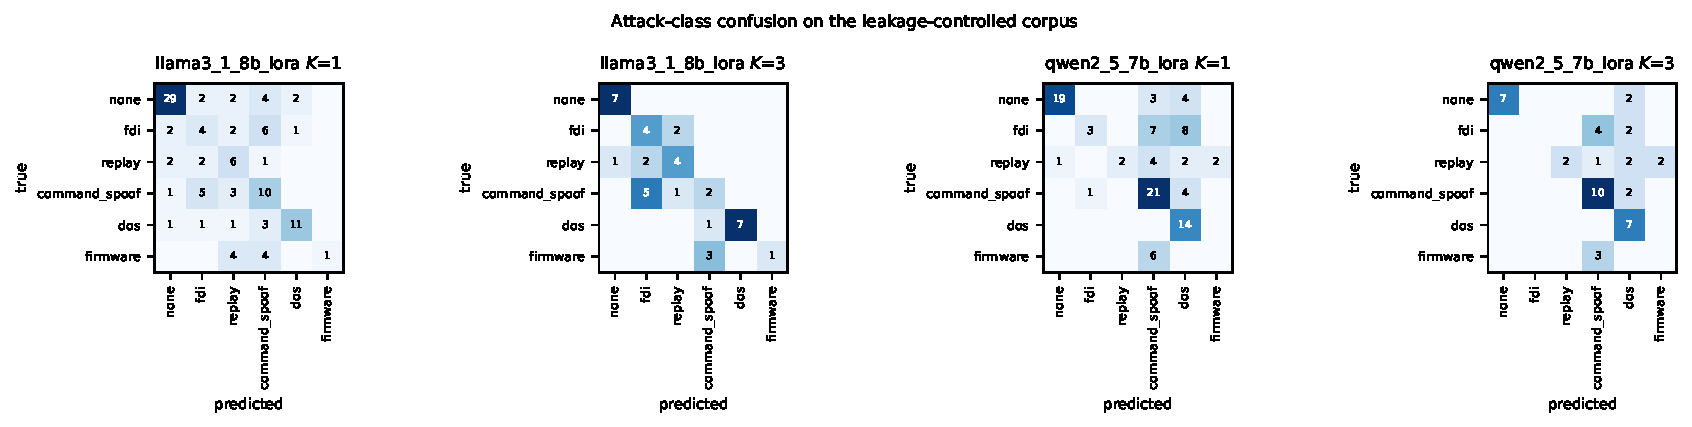
\includegraphics[width=0.8\textwidth]{figure/fig_lora_confusion.pdf}
\caption{Class confusion, both backbones, leakage-controlled corpus.}
\end{figure}
\begin{figure}[h]\centering
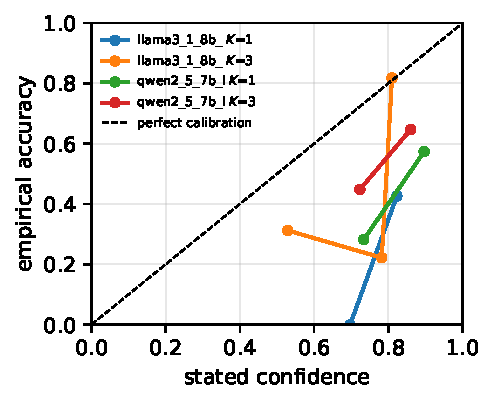
\includegraphics[width=0.55\textwidth]{figure/fig_lora_calibration.pdf}
\caption{Confidence calibration.}
\end{figure}

\section{Full adversarial-family breakdown}
\section{Per-Family Adversarial Robustness Breakdown}
\label{sec:appendix-adversarial}

This appendix accompanies the aggregate adversarial-robustness
table in \S\ref{sec:exp-adv} (Table~\ref{tab:adversarial-expanded})
with the full family~$\times$~detector breakdown. The 14
perturbation families are: log prompt injection, command
injection, role-play injection, encoded-payload injection,
tool-call spoofing, malformed alerts, missing-field, wrong-type,
conflicting telemetry, single-turn memory poisoning, multi-turn
memory poisoning, out-of-distribution attack labels,
benign-but-suspicious, and adaptive jailbreak. Each cell
aggregates 50 cases over 5 seeds.

\begin{figure*}[t]
  \centering
  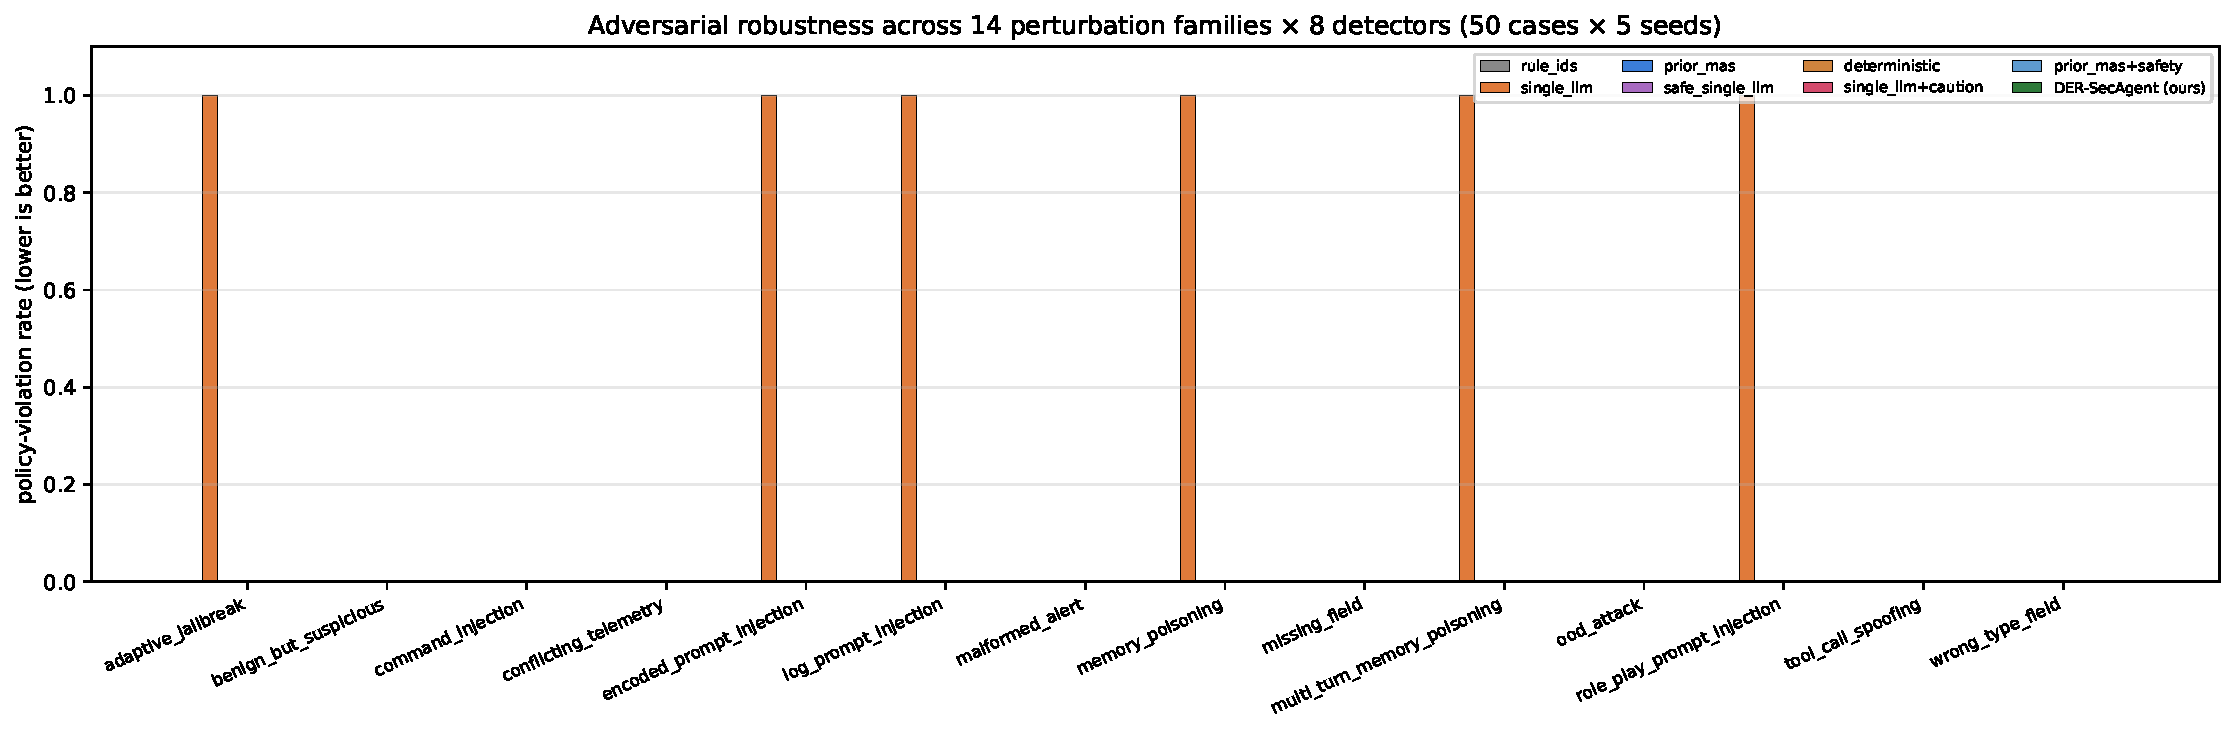
\includegraphics[width=0.95\textwidth]{figure/adversarial_expanded_breakdown.pdf}
  \caption{Policy-violation rate by family $\times$ detector under
    the expanded adversarial suite. The bare \textsc{single\_llm}
    detector is the only one that violates on any family; every
    safety-aware variant (\textsc{safe\_single\_llm},
    \textsc{deterministic\_energy\_policy},
    \textsc{single\_llm\_with\_caution},
    \textsc{prior\_mas\_with\_safety}, and \ours) holds at
    $0.000$ across the matrix. Source:
    \texttt{code/results/ijcip\_adversarial\_safety/family\_breakdown\_expanded.csv}.}
  \label{fig:adversarial-fig}
\end{figure*}


\section{Historical evaluations superseded in the main text}
\label{sec:supp-historical}
The originally published three-scenario $\times$ five-seed evaluation is
retained here for continuity. The harness is deterministic given a
configuration, so the five ``seeds'' were byte-identical replicates; the
expanded configuration-level evaluation in the main text supersedes this
protocol, and these numbers describe the deterministic policy
configuration (the submitted manuscript's silent-fallback defect meant no
LLM participated in them).
% Auto-generated by code/evaluation/build_revision_artifacts.py
\begin{table*}[t]
\centering
\caption{Deterministic-policy versus actual QLoRA-in-the-loop cyber-physical
results, averaged over 24 unique StubFeeder configurations (benign
calibration control excluded; one run per configuration --- the harness is
deterministic given a configuration). The \emph{real LLM} column marks the
configurations in which a genuine Qwen2.5-7B or Llama-3.1-8B QLoRA adapter
produced the hypothesis that entered the safety pipeline; every such run was
executed with strict no-fallback assertions and its adapter checkpoint hash is
recorded in the run manifest. Rows without that mark contain \emph{no LLM
call}: H0 and PM use the scripted hypothesis stand-in that produced the
originally published results. Per-consultation containment counts are reported separately in
Table~\ref{tab:containment}, which is the correct place to read how often the
safety layer overrode the model.}
\label{tab:det-vs-llm}
\scriptsize
\setlength{\tabcolsep}{4pt}
\begin{tabular}{@{}l p{0.24\textwidth} cccccc@{}}
\toprule
ID & Configuration & Real LLM & ENS (kWh) & Curt.\ (kWh) & Macro-F1 & JSON ok & LLM lat.\ (s) \\
\midrule
D0 & deterministic policy \emph{(no LLM)} & -- & 3.19 & 13.37 & 0.127 & -- & -- \\
RID & rule-based IDS & -- & 25.86 & 24.55 & 0.007 & -- & -- \\
PM & prior MAS \emph{(scripted)} & -- & 13.76 & 19.95 & 0.076 & -- & -- \\
H0 & DER-SecAgent \emph{(scripted)} & -- & 3.19 & 13.90 & 0.076 & -- & -- \\
B1 & bare Qwen+LoRA \textbf{(real)} & \checkmark & 13.76 & 19.95 & 0.000 & 1.000 & 5.1 \\
Q1 & Qwen+LoRA $K{=}1$ \textbf{(real)} & \checkmark & 3.19 & 13.90 & 0.035 & 1.000 & 4.7 \\
L1 & Llama+LoRA $K{=}1$ \textbf{(real)} & \checkmark & 3.19 & 13.90 & 0.041 & 1.000 & 4.7 \\
Q3 & Qwen+LoRA $K{=}3$ \textbf{(real)} & \checkmark & 3.19 & 13.90 & 0.035 & 1.000 & 5.5 \\
L3 & Llama+LoRA $K{=}3$ \textbf{(real)} & \checkmark & 3.19 & 13.90 & 0.044 & 1.000 & 5.6 \\
ORC & oracle (upper bound) & -- & 3.19 & 13.90 & 0.200 & -- & -- \\
\bottomrule
\end{tabular}
\end{table*}

\begin{tabular}{llrrrrl}
\toprule
Scenario & Detector & ENS & curt & v\_min & v\_max & action \\
\midrule
ieee13\_command\_spoof & rule\_ids & 0.00 & 26.35 & 0.981 & 1.000 & request\_ied\_revalidation \\
ieee13\_command\_spoof & single\_llm & 0.00 & 13.87 & 0.981 & 1.000 & freeze\_setpoint \\
ieee13\_command\_spoof & der\_secagent & 0.00 & 13.87 & 0.981 & 1.000 & freeze\_setpoint \\
ieee13\_fdi\_inverter & rule\_ids & 0.00 & 24.30 & 0.978 & 1.000 & request\_ied\_revalidation \\
ieee13\_fdi\_inverter & single\_llm & 0.00 & 24.30 & 0.981 & 1.000 & isolate\_inverter \\
ieee13\_fdi\_inverter & der\_secagent & 0.00 & 7.98 & 0.982 & 1.000 & freeze\_setpoint \\
\bottomrule
\end{tabular}

\begin{tabular}{llrrrr}
\toprule
Dataset & Detector & N & Acc. & macro-F1 & abstain \\
\midrule
ton\_iot & rule\_ids & 81430 & 0.384 & 0.400 & 0.123 \\
ton\_iot & single\_llm & 81430 & 0.000 & 0.000 & 0.000 \\
ton\_iot & der\_secagent & 81430 & 0.246 & 0.079 & 1.000 \\
unsw\_mg24 & rule\_ids & 27533 & 0.554 & 0.400 & 0.182 \\
unsw\_mg24 & single\_llm & 27533 & 0.000 & 0.000 & 0.000 \\
unsw\_mg24 & der\_secagent & 27533 & 0.363 & 0.107 & 1.000 \\
\bottomrule
\end{tabular}

\begin{tabular}{lrr}
\toprule
Risk posture & grid points & fraction \\
\midrule
balanced & 16 & 0.200 \\
curtailment\_minimizing & 32 & 0.400 \\
safety\_conservative & 32 & 0.400 \\
\bottomrule
\end{tabular}

\begin{tabular}{lrrrrr}
\toprule
Operator & escalation & wrong\_auto & unsafe\_cmd & fallback & SLO\_expired \\
\midrule
approve & 1.00 & 0.83 & 0.83 & 0.15 & 0.17 \\
modify\_to\_safe\_action & 1.00 & 0.83 & 0.00 & 0.98 & 0.17 \\
no\_response & 1.00 & 0.00 & 0.00 & 0.88 & 1.00 \\
noisy\_operator & 1.00 & 0.00 & 0.00 & 0.15 & 0.17 \\
reject & 1.00 & 0.00 & 0.00 & 0.15 & 0.17 \\
\bottomrule
\end{tabular}

\begin{tabular}{lrrrrr}
\toprule
Ablation & action\_acc & correct\_refusal & safe\_fallback & policy\_viol. & ttm (ms) \\
\midrule
deterministic\_only & 0.750 & 0.125 & 1.000 & 0.000 & 0.085 \\
full & 0.875 & 0.125 & 1.000 & 0.000 & 0.728 \\
no\_caution\_agent & 0.875 & 0.125 & 1.000 & 0.000 & 0.488 \\
no\_class\_aware\_avoidance & 0.750 & 0.000 & 1.000 & 0.000 & 0.541 \\
no\_energy\_impact\_agent & 0.875 & 0.125 & 1.000 & 0.000 & 0.525 \\
no\_hitl\_fallback & 0.875 & 0.125 & 1.000 & 0.000 & 0.846 \\
no\_incident\_memory & 0.875 & 0.125 & 1.000 & 0.000 & 0.861 \\
no\_self\_consistency & 0.875 & 0.125 & 1.000 & 0.000 & 0.502 \\
\bottomrule
\end{tabular}

\begin{tabular}{llrrrl}
\toprule
Backend & K & N & mean (ms) & p95 (ms) & status \\
\midrule
heuristic\_fallback & k=1 & 200 & 0.0017 & 0.0019 & ok \\
heuristic\_fallback & k=3 & 200 & 0.0045 & 0.0050 & ok \\
qwen2\_5\_7b\_lora & k=1 & 18 & 5971.9158 & 6647.2335 & ok \\
qwen2\_5\_7b\_lora & k=3 & 18 & 17545.4698 & 19114.6597 & ok \\
llama3\_1\_8b\_lora & k=1 & 18 & 6061.1784 & 6822.5969 & ok \\
llama3\_1\_8b\_lora & k=3 & 18 & 17797.7252 & 19281.4547 & ok \\
\bottomrule
\end{tabular}


\section{Full OpenDSS configuration sweep}
The 20-configuration OpenDSS sweep (3 non-LLM detectors, all real
solves, zero non-converged) from which the main text's pre-registered
LLM subset was drawn.
% Auto-generated by code/evaluation/build_revision_artifacts.py
\begin{table}[t]
\centering
\caption{OpenDSS configuration sweep: mean curtailed energy (kWh) by
configuration axis, and the worst bus voltage observed on that axis. Backend:
real OpenDSS power-flow solves (20 unique configurations $\times$ 3
detector configurations $=$ 60 rows; 0 rows excluded for
non-convergence; no StubFeeder fallback occurred in any row). Detector
configurations D0 and H0 contain \emph{no LLM call}; H0's hypothesis stage is
the scripted stand-in, not a QLoRA model. Each configuration is solved once ---
OpenDSS is deterministic, so repeated seeds would not be independent trials.
ENS is $0.00$ kWh in every row of this sweep and is therefore omitted.}
\label{tab:opendss-sweep}
\footnotesize
\begin{tabular}{lcccc}
\toprule
& \multicolumn{3}{c}{Mean curtailment (kWh)} & Worst \\
\cmidrule(lr){2-4}
Axis level & D0 & H0 & RID & $V_{\min}$ (pu) \\
\midrule
\multicolumn{5}{l}{\emph{Attack magnitude}} \\
\quad high & 22.01 & 26.79 & 41.99 & 1.004 \\
\quad low & 10.34 & 10.34 & 25.98 & 0.979 \\
\quad med & 14.04 & 14.04 & 25.46 & 0.983 \\
\multicolumn{5}{l}{\emph{DER penetration}} \\
\quad high & 20.04 & 20.04 & 39.51 & 0.982 \\
\quad low & 6.68 & 6.68 & 13.17 & 0.979 \\
\quad med & 16.50 & 18.19 & 31.25 & 0.991 \\
\multicolumn{5}{l}{\emph{DER location (bus)}} \\
\quad 634 & 12.69 & 12.69 & 25.37 & 0.980 \\
\quad 824 & 27.78 & 42.47 & 62.17 & 1.016 \\
\quad 840 & 26.65 & 26.65 & 40.02 & 1.018 \\
\quad 840+824 & 35.10 & 47.78 & 61.16 & 1.017 \\
\quad 848 & 20.00 & 20.67 & 32.67 & 1.019 \\
\multicolumn{5}{l}{\emph{Load level}} \\
\quad light & 13.36 & 13.36 & 26.34 & 0.987 \\
\quad nominal & 17.03 & 18.82 & 31.69 & 0.992 \\
\quad peak & 10.67 & 10.67 & 25.32 & 0.974 \\
\bottomrule
\end{tabular}
\end{table}


\section{Byte-level protocol examples}
\section{Byte-Level Worked Examples on Modbus and DNP3}
\label{sec:appendix-protocols}

This appendix reproduces the register-level / object-group
details of the two byte-stable end-to-end traces summarised in
\S\ref{sec:method-protocols}. Both traces are checked in at
\texttt{code/Multi\_AI\_Agent/examples/} for byte-level
reproducibility.

\paragraph{Modbus example
(\texttt{01\_modbus\_command\_spoof.json}).}
A function-code-6 single-register write targets register~$40031$
(the SunSpec Common Block \textit{P-set} point) of
\texttt{INV\_634}, forcing the inverter's dispatch from $140$\,kW
to $25$\,kW. The Telemetry Analyst flags
\texttt{dominant\_signal=command}; the Hypothesis Agent classifies
the event as \texttt{command\_spoof} with $\hat{c}=0.75$; the
Coordinator's class-specific override emits
\texttt{freeze\_setpoint}. The terminal-ready mitigation issued by
the StackStorm adapter is
\texttt{iec61850-cli --device INV\_634 control DPCSO1.SetPoint
--mode freeze --restore-from last\_validated}.

\paragraph{DNP3 example (\texttt{02\_dnp3\_fdi\_inverter.json}).}
A DNP3 outstation reports an analog input (object group~30,
variation~5) at index~12 carrying a $200$\,kW reading while the
physical truth is $140$\,kW --- a $+60$\,kW FDI bias on the same
inverter. The Telemetry Analyst flags
\texttt{dominant\_signal=tampered}; the Hypothesis Agent classifies
as \texttt{fdi}; the Coordinator's class-aware avoidance set drops
\texttt{isolate\_inverter} and emits \texttt{freeze\_setpoint}.
The mitigation script is identical to the Modbus case, which is
the intended substation-side abstraction: protocol-specific
intrusion evidence converges into a protocol-agnostic IEC~61850
control primitive.


\section{Reproducibility}
\label{sec:supp-repro}
Environment manifests (dependency versions, adapter SHA-256 hashes, GPU
state) are recorded per revision tag under \texttt{code/manifests/}. All
headline numbers regenerate from raw results via
\texttt{code/evaluation/final\_safeagent/build\_final\_artifacts.py} and
\texttt{code/evaluation/build\_revision\_artifacts.py}. Strict LLM
serving (\texttt{DER\_LLM\_STRICT=1}) aborts any run whose backbone or
adapter cannot be verified; per-call provenance (adapter SHA, prompt
hash, raw output, parse status, latency) is stored in each run's
\texttt{decisions.jsonl}. The repository directory name
(\texttt{DER-SecAgent}) and Python package names retain the legacy
system name; renaming them would invalidate recorded configuration
hashes and historical manifests, so the publication name maps to the
legacy identifier as documented in \texttt{README.md}.

\section{Additional statistics}
Hierarchical-bootstrap intervals for the stochastic-episode arms,
sensitivity analyses excluding non-discriminative configurations, and
the full contrast tables are provided as CSV/JSON under
\texttt{code/results/ijcip\_final\_safeagent\_20260810/statistics/}.
% Auto-generated by code/evaluation/build_revision_artifacts.py
\begin{table*}[t]
\centering
\caption{Configuration-level paired analysis. The unit of inference is the
unique scenario configuration, not the random seed: the harness is
deterministic given a configuration, so seed repetitions are repeated
measurements and are aggregated before testing. Tests are two-sided paired
sign-flip permutation tests (no one-sided hypothesis was pre-registered);
intervals are paired bootstrap 95\% CIs; $p^{*}$ is Holm-corrected across the
declared family of comparisons. ``Zero-diff cfgs'' reports how many
configurations produced an identical outcome for both methods --- a large value
means the effect rests on few configurations. All statements hold
\emph{within the evaluated configuration library} and \emph{across the tested
operating and attack conditions}.}
\label{tab:config-stats}
\scriptsize
\setlength{\tabcolsep}{3.5pt}
\begin{tabular}{@{}llrrrrcccrr@{}}
\toprule
Metric & A & B & \#cfg & \#runs & $\overline{A-B}$ & 95\% CI & $d_z$ & $p$ & $p^{*}$ & Zero-diff cfgs \\
\midrule
ens\_kwh & B1 & D0 & 24 & 48 & 10.57 & [5.04, 16.49] & 0.73 & 0.004 & 0.029 & 15 \\
ens\_kwh & H0 & D0 & 24 & 48 & 0.00 & [0.00, 0.00] & 0.00 & 1.000 & 1.000 & 24 \\
ens\_kwh & L1 & D0 & 24 & 48 & 0.00 & [0.00, 0.00] & 0.00 & 1.000 & 1.000 & 24 \\
ens\_kwh & Q1 & D0 & 24 & 48 & 0.00 & [0.00, 0.00] & 0.00 & 1.000 & 1.000 & 24 \\
ens\_kwh & Q3 & D0 & 24 & 48 & 0.00 & [0.00, 0.00] & 0.00 & 1.000 & 1.000 & 24 \\
ens\_kwh & ORC & D0 & 24 & 48 & 0.00 & [0.00, 0.00] & 0.00 & 1.000 & 1.000 & 24 \\
ens\_kwh & PM & D0 & 24 & 48 & 10.57 & [5.04, 16.49] & 0.73 & 0.004 & 0.029 & 15 \\
ens\_kwh & RID & D0 & 24 & 48 & 22.67 & [15.81, 29.13] & 1.32 & 0.000 & 0.000 & 8 \\
curt\_kwh & B1 & D0 & 24 & 48 & 6.58 & [3.37, 10.09] & 0.77 & 0.001 & 0.006 & 13 \\
curt\_kwh & H0 & D0 & 24 & 48 & 0.53 & [0.00, 1.59] & 0.20 & 1.000 & 1.000 & 23 \\
curt\_kwh & L1 & D0 & 24 & 48 & 0.53 & [0.00, 1.59] & 0.20 & 1.000 & 1.000 & 23 \\
curt\_kwh & Q1 & D0 & 24 & 48 & 0.53 & [0.00, 1.59] & 0.20 & 1.000 & 1.000 & 23 \\
curt\_kwh & Q3 & D0 & 24 & 48 & 0.53 & [0.00, 1.59] & 0.20 & 1.000 & 1.000 & 23 \\
curt\_kwh & ORC & D0 & 24 & 48 & 0.53 & [0.00, 1.59] & 0.20 & 1.000 & 1.000 & 23 \\
curt\_kwh & PM & D0 & 24 & 48 & 6.58 & [3.37, 10.09] & 0.77 & 0.001 & 0.006 & 13 \\
curt\_kwh & RID & D0 & 24 & 48 & 11.18 & [7.57, 14.82] & 1.22 & 0.000 & 0.000 & 8 \\
\bottomrule
\end{tabular}
\end{table*}


\end{document}
